\renewcommand\thesection{\arabic{section}}
\renewcommand\thesubsection{\thesection.\arabic{subsection}}


\textbf{Goal}:

To segment the detected surface of wooden beams, especially give the difference between the main surface and the others; (ideal output like Figure~\ref{fig:mock1})

\hspace*{\fill}


\begin{figure}[ht]
  \centering
    \begin{subfigure}[b]{0.4\textwidth}
      \centering
        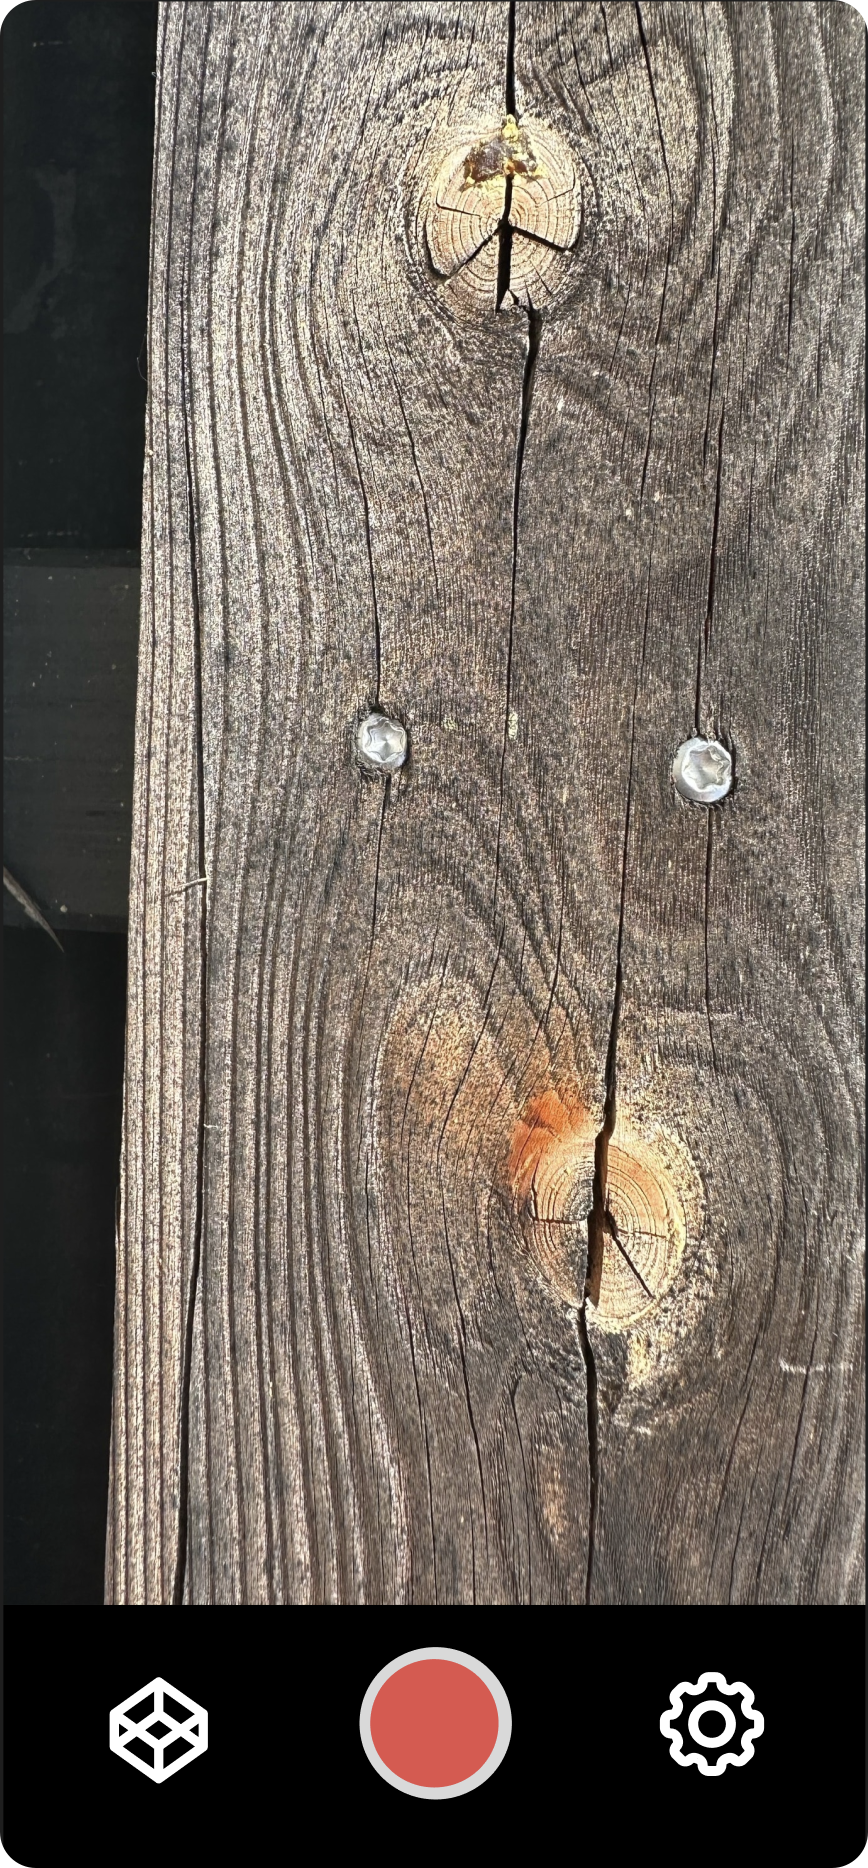
\includegraphics[width=0.5\textwidth]{Master Thesis/Images/Section_3/Mock/3-Mock1.png}
    \end{subfigure}
    \begin{subfigure}[b]{0.4\textwidth}
      \centering
        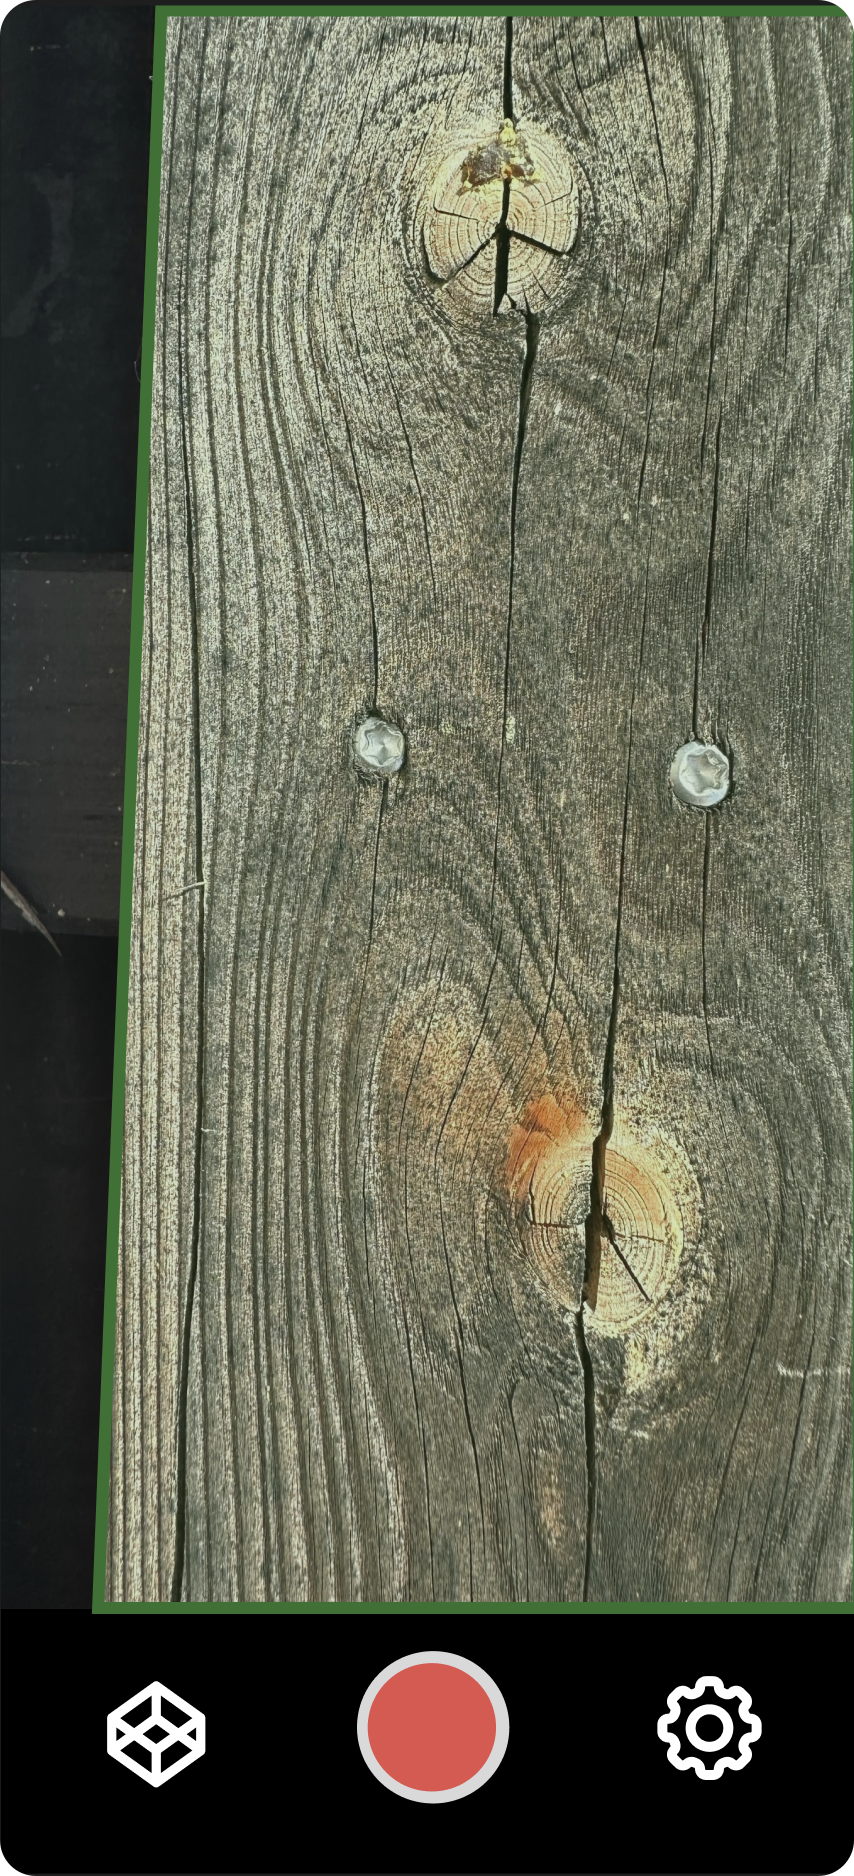
\includegraphics[width=0.5\textwidth]{Master Thesis/Images/Section_3/Mock/3-Mock2.png}
    \end{subfigure}
  \caption{Mocked-up output through segmentation of wooden beams on the iPhone}   
\label{fig:mock1}
\end{figure}  

\textbf{Data set}:

The data set for this step will be captured through different wooden constructions which the main surface (target surface) and the rest surfaces will be masked. Currently, there are more than 800 captured images for segmentation of wooden beams to be annotated.

\hspace*{\fill}

\newpage
\textbf{Potential methods}:

Several models will be considered to achieve a valuable performance for the segmentation. Stat-of-art models like Segment Anything~\citep{kirillov2023segany}(Test in Figure~\ref{fig:sam_test}), Detectron2~\citep{wu2019detectron2} or Mask R-CNN~\citep{matterport_maskrcnn_2017} are expected to support this step. However, all models need to be fine-tuned using the mentioned datasets to hopefully segment the main target wooden beams and properly be modified to fit the final workflow.

\hspace*{\fill}

\textbf{Output}:

Output will be the segmented single image and position of segmented target area.

\begin{figure}[ht]
  \centering
    \begin{subfigure}[b]{0.3\textwidth}
      \centering
        \includegraphics[width=\textwidth,height=4cm,keepaspectratio=false]{Master Thesis/Images/Section_3/SAM/3_sam_test_1.png}
    \end{subfigure}
    \hspace{1cm}
    \begin{subfigure}[b]{0.3\textwidth}
      \centering
        \includegraphics[width=\textwidth,height=4cm,keepaspectratio=false]{Master Thesis/Images/Section_3/SAM/3_sam_test_2.png}
    \end{subfigure}
  \caption{Examples of segmentation on wooden beams using SAM (segment anything)}
\label{fig:sam_test}
\end{figure}

\hspace*{\fill}

% \textbf{Potential challenges}:\\
% - \\
% - 313\\
% - qweq\\